\section{SAT model}

% The resolution of the problem is approached following two models.

% \begin{itemize}
%     \item \textbf{Unified model}:
%     based on the definition of two decision variables \texttt{assignments} and \texttt{paths}.
%     \item \textbf{Matrix model}:
%     based on the definition of one decision variable $X$.
% \end{itemize}

% Some modifications were applied to those model in order to visualize eventual differences in terms of performances.

% The discussion is going to be much more focused on the Unified model just to mantain a logical thread within the explication of models used for other solvers.

% \subsection{Unified Model}

% \paragraph*{General Definition}
% The Unified model aims to find the correct assignment to both decision variables, in such a way that it satisfy all constraints.\\
% The idea behind this kind of model is based on the separation of the two task just specified in one.

% \paragraph*{Original Workflow}
% The original workflow follows the next steps:
% \begin{enumerate}
%     \item find satisfying values for the \texttt{assignments} variable, else end the algorithm
%     \item find satisfying values for the \texttt{paths} variable, else proceed to step $4$
%     \item repeat step $2$ to find a new optimized solution,
%     \item repeat step $1$ just to find another assignment
% \end{enumerate}

% \paragraph*{New Workflow}
% The new algorithm simply tries to optimize the assignment to both variable.

% \paragraph*{Pro}
% The model was designed to improve certain intrinsic problems of the definition of a problem through SAT:
% \begin{itemize}
%     \item \textbf{Specificity of constraints}: constraining much more the assignments of the two variable guarantes to mantain lower width of exploration of the resolution tree.
% \end{itemize} 

% \paragraph*{Contro}
% The model falls into a few issues such:

% \begin{itemize}
%     \item \textbf{Dimension}: being based on two decision variables, the dimension of the problem scale exponentially with them. \footnote{The scaling dimension of the problem implies higher needs of time to build the model.}
% \end{itemize}

\subsection{Decision variables}

For SAT, we defined two different models:
\begin{description}
    \item[Unified model] based on the definition of the two decision variables $A$ (\texttt{assignments} in Z3) and $P$ (\texttt{paths} in Z3) as defined in \Cref{sec:intro}.

    \item[Matrix model] based on the definition of a single matrix $X$ such that $X\texttt{[$c$, $p$, $k$]} = 1$ iff courier $c$ delivers item $p$ as its $k$-th package.
\end{description}

Our discussion will be focused on the former to maintain coherence with the models defined in the other methods and obtain more comparable results. Its decision variables are the following:

\begin{itemize}
    \item $A$ is an $n \times m$ matrix such that $A\texttt{[$p$, $c$]} = 1$ iff courier $c$ delivers item $p$.

    \item $P$ is an $m \times (n+1) \times (n+1)$ matrix such that $P\texttt{[$c$, $loc_1$, $loc_2$]} = 1$ iff courier $c$ moves from location $loc_1$ to $loc_2$.

    \item $U$ is an $m \times n \times n$ matrix to implement MTZ subtour elimination \cite{mtz_subtour}. $U\texttt{[$c$, $p$, $k$]} = 1$ iff for the courier $c$ the item $p$ is delivered as the $k$-th.
\end{itemize}

\subsection{Objective function}

The objective function is computed as follows:
\begin{equation}
    \label{eq:obj_fun}
    \max_{c \in [1, m]}
    \sum_{loc_1=1}^{n+1} \sum_{\substack{loc_2=1,\\loc_2 \neq loc_1}}^{n+1} \texttt{D[$loc_1$, $loc_2$]} \cdot P\texttt{[$c$, $loc_1$, $loc_2$]}
\end{equation}


\subsection{Constraints}

\paragraph*{Assignment related constraints}

\begin{itemize}
    \item Capacity constraint:
    \begin{itemize}
        \item The sum of the size of the items delivered by a courier must be within its load limit:
        \begin{equation}
            \label{eq:capacity1}
            \forall c \in [1, m]:
            \sum_{p=1}^{n} A\texttt{[$p$, $c$]} \cdot s\texttt{[$p$]} \leq \texttt{$l$[$c$]}
        \end{equation}
        \item Each item must be delivered by only one courier:
        \begin{equation}
            \label{eq:capacity2}
            \forall p \in [1, n], \exists! c \in [1, m]: A\texttt{[$p$, $c$]} = 1
        \end{equation}
    \end{itemize}
\end{itemize}

\paragraph*{Path related constraints}

\begin{itemize}
    \item General path constraints
    \begin{itemize}
        \item If a courier delivers at least one package, there must exist a destination from $\texttt{DEPOT}=n+1$ with its value set to true, else it stays in \texttt{DEPOT}:
            \begin{equation}
                \label{eq:gen_path_constr1}
                \makebox[\displaywidth]{$
                    \forall c \in [1, m],
                    \forall p \in [1, n]:
                    \begin{cases}
                        P\texttt{[$c$, DEPOT, DEPOT]}=0 & \text{if } \sum_{p=1}^{n} A\texttt{[$p$, $c$]} \geq 1\\
                        P\texttt{[$c$, DEPOT, DEPOT]}=1 & \text{if } \sum_{p=1}^{n} A\texttt{[$p$, $c$]} = 0 % or otherwise
                    \end{cases}
                $}
            \end{equation}
        
        \item If a courier delivers item $p$, its successor in $P$ must be different from $p$:
        \begin{equation}
            \label{eq:gen_path_constr2}
            \forall c \in [1, m],
            \forall p \in [1, n]:
            \begin{cases}
                P\texttt{[$c$, $p$, $p$]}=0 & \text{if } A\texttt{[$p$, $c$]}=1\\
                P\texttt{[$c$, $p$, $p$]}=1 & \text{if } A\texttt{[$p$, $c$]}=0 % or otherwise
            \end{cases}
        \end{equation}

        \item For each courier, there is exactly one successor location:
        \begin{equation}
            \label{eq:gen_path_constr3}
            \forall c \in [1, m],
            \forall loc_1 \in [1, n+1]:
            \quad
            \sum_{loc_2=1}^{n+1} P\texttt{[$c$, $loc_1$, $loc_2$]} = 1
        \end{equation}

        \item For each courier, there is exactly one predecessor location:
        \begin{equation}
            \label{eq:subtour_constr1}
            \forall c \in [1, m],
            \forall loc_2 \in [1, n+1]:
            \quad
            \sum_{loc_1=1}^{n+1} P\texttt{[$c$, $loc_1$, $loc_2$]} = 1
        \end{equation}
    \end{itemize}

    \item MTZ subtour elimination constraints
        \begin{itemize}
            \item $U$ relative to the first item $p$ of the path of a courier $c$ must be 1:
            \begin{equation}
                \label{eq:subtour_constr2}
                \forall c \in [1, m],
                \forall p \in [1, n]:
                P\texttt{[$c$, DEPOT, $p$]}=1
                \Rightarrow
                U\texttt{[$c$, $p$, $1$]}=1
            \end{equation}
            
            \item $U$ relative to an item $j$ delivered after $i$ should be greater ($U_j \geq U_i+1$):
            \begin{equation}
                \makebox[\displaywidth]{$
                    \label{eq:subtour_constr3}
                    \forall c \in [1, m], \ \forall i, j, k \in [1, n]:
                    \left(P\texttt{[$c$, $i$, $j$]} \land U\texttt{[$c$, $i$, $k$]}\right) \Rightarrow
                    \sum_{l=k+1}^{n} U\texttt{[$c$, $j$, $l$]} = 1
                $}
            \end{equation}
            
            \item $U$ relative to an item $p$ of a courier must have exactly one value associated:
            \begin{equation}
                \label{eq:subtour_constr4}
                \forall c \in [1, m],
                \forall p \in [1, n]:
                \sum_{k=1}^{n} U\texttt{[$c$, $p$, $k$]} = 1
            \end{equation}

            \item MTZ formulation:
            \begin{equation}
                \label{eq:subtour_constr5}
                \makebox[\displaywidth]{$
                    \begin{split}
                        &\forall c \in [1, m], \ \forall i, j, k_1, k_2 \in [1, n]: \\
                        &(U\texttt{[$c$, $i$, $k_1$]} \land U\texttt{[$c$, $j$, $k_2$]})\Rightarrow
                        (k_1 - k_2 + 1) \leq (n-1) \cdot (1 - P\texttt{[$c$, $i$, $j$]})
                    \end{split}
                $}
            \end{equation}
        \end{itemize}
\end{itemize}

\subsubsection{Symmetry breaking constraint}

A possible way to reduce tree exploration is to introduce symmetry breaking constraints. In particular, for SAT, we experimented only with the one defined in \Cref{eq:cp_symm_packs}.


\subsection{Validation}

\subsubsection{Experimental design}

Some modifications were applied to the basic model in order to visualize possible differences in performance.
The original Unified Model was modified in three different versions:
\begin{enumerate*}[label=(\roman*)]
    \item with Symmetry Breaking Constraints,
    \item with Cumulative Constraint Application,
    \item with the Heule Encoding for \texttt{at\_most\_one()}.
\end{enumerate*}

To optimize the objective function, we follow the standard approach of iteratively solving the problem and imposing as new constraint the fact that a new objective must be lower than the one already found.


\subsubsection{Experimental results}

As we can notice from \Cref{tab:sat_results}, the performances were not very much different from the basic model. Only in the first 10 instances it has been possible to reach at least a suboptimal solution, while for the remaining ones the construction of the model required too much time causing to exceed the timeout limit. Symmetry breaking also did not contribute to improve the results. 

\begin{table}[H]
    \centering
    \caption{Objective value through instances}
    \label{tab:sat_results}
    \centerline{
        \begin{tabular}{cccccc}
            \toprule
            Id & un-model & un-symm-model & un-cum-constr-model & un-heule-enc-model & matrix-model \\ 
            \midrule
            1 & \textbf{14} &       \textbf{14} &   \textbf{14} &   \textbf{14} &   \textbf{14} \\ 
            2 & \textbf{226} &      \textbf{226} &  \textbf{226} &  \textbf{226} &  \textbf{226} \\ 
            3 & \textbf{12} &       \textbf{12} &   \textbf{12} &   \textbf{12} &   \textbf{12} \\ 
            4 & \textbf{220} &      \textbf{220} &  \textbf{220} &  \textbf{220} &  \textbf{220} \\ 
            5 & \textbf{206} &      \textbf{206} &  \textbf{206} &  \textbf{206} &  \textbf{206} \\ 
            6 & \textbf{322} &      \textbf{322} &  \textbf{322} &  \textbf{322} &  \textbf{322} \\ 
            7 & 232 &       238 &   222 &   296 &   292 \\ 
            8 & \textbf{186} &      \textbf{186} &  \textbf{186} &  \textbf{186} &  \textbf{186} \\ 
            9 & \textbf{436} &      \textbf{436} &  \textbf{436} &  \textbf{436} &  \textbf{436} \\ 
            10 & \textbf{244} &     \textbf{244} &  \textbf{244} &  \textbf{244} &  \textbf{244} \\ 
            \bottomrule
        \end{tabular}
    }
\end{table}


\begin{figure}[h]
    \centering
    \begin{subfigure}{0.49\linewidth}
        \centering
        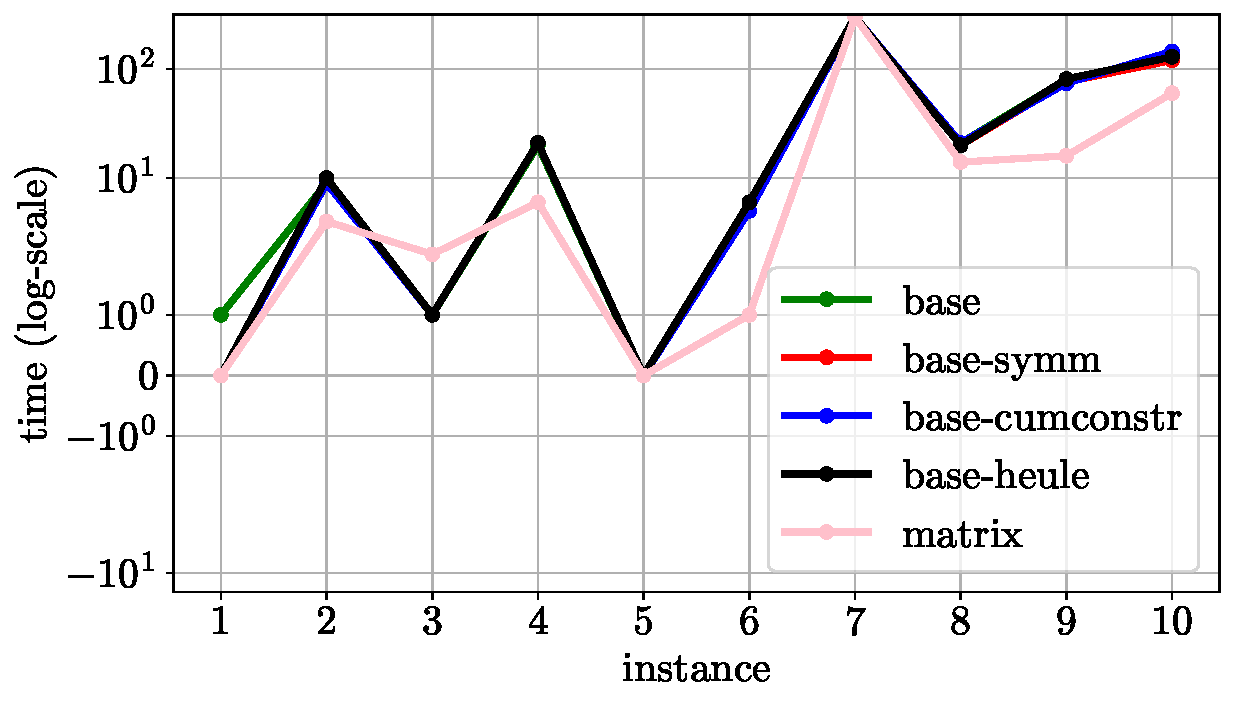
\includegraphics[width=\linewidth]{img/sat/time.pdf}
        \caption{Resolution time}
    \end{subfigure}
    \hfill
    \centering
    \begin{subfigure}{0.49\linewidth}
        \centering
        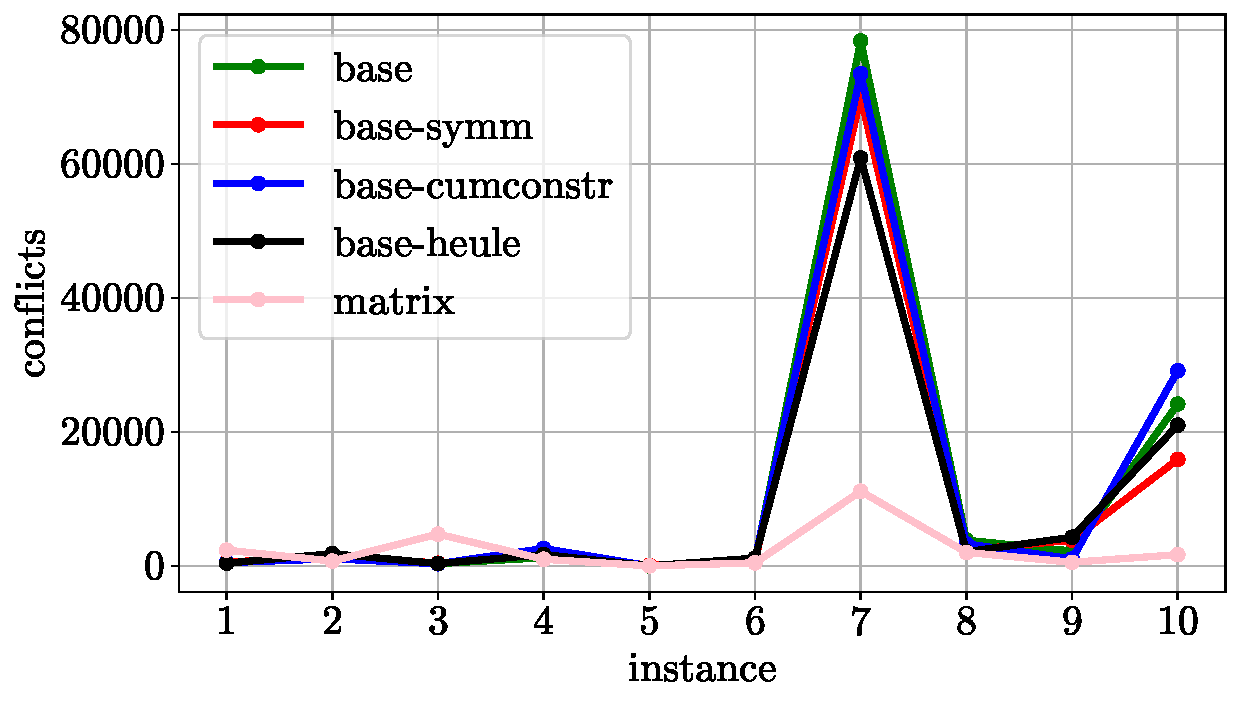
\includegraphics[width=\linewidth]{img/sat/conflicts.pdf}
        \caption{Number of conflicts}
    \end{subfigure}
    \\
    \centering
    \begin{subfigure}{0.49\linewidth}
        \centering
        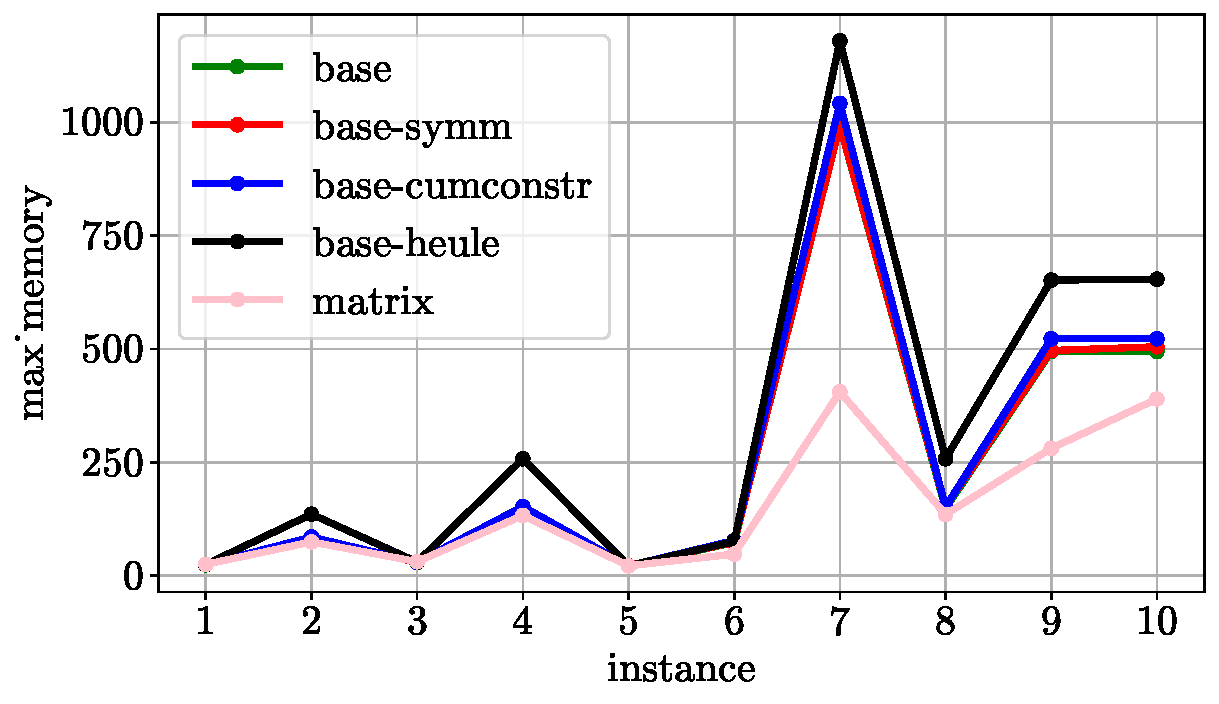
\includegraphics[width=\linewidth]{img/sat/max_memory.pdf}
        \caption{Maximum amount of memory required}
    \end{subfigure}
    % \hfill
    % \centering
    % \begin{subfigure}{0.49\linewidth}
        % \centering
        % 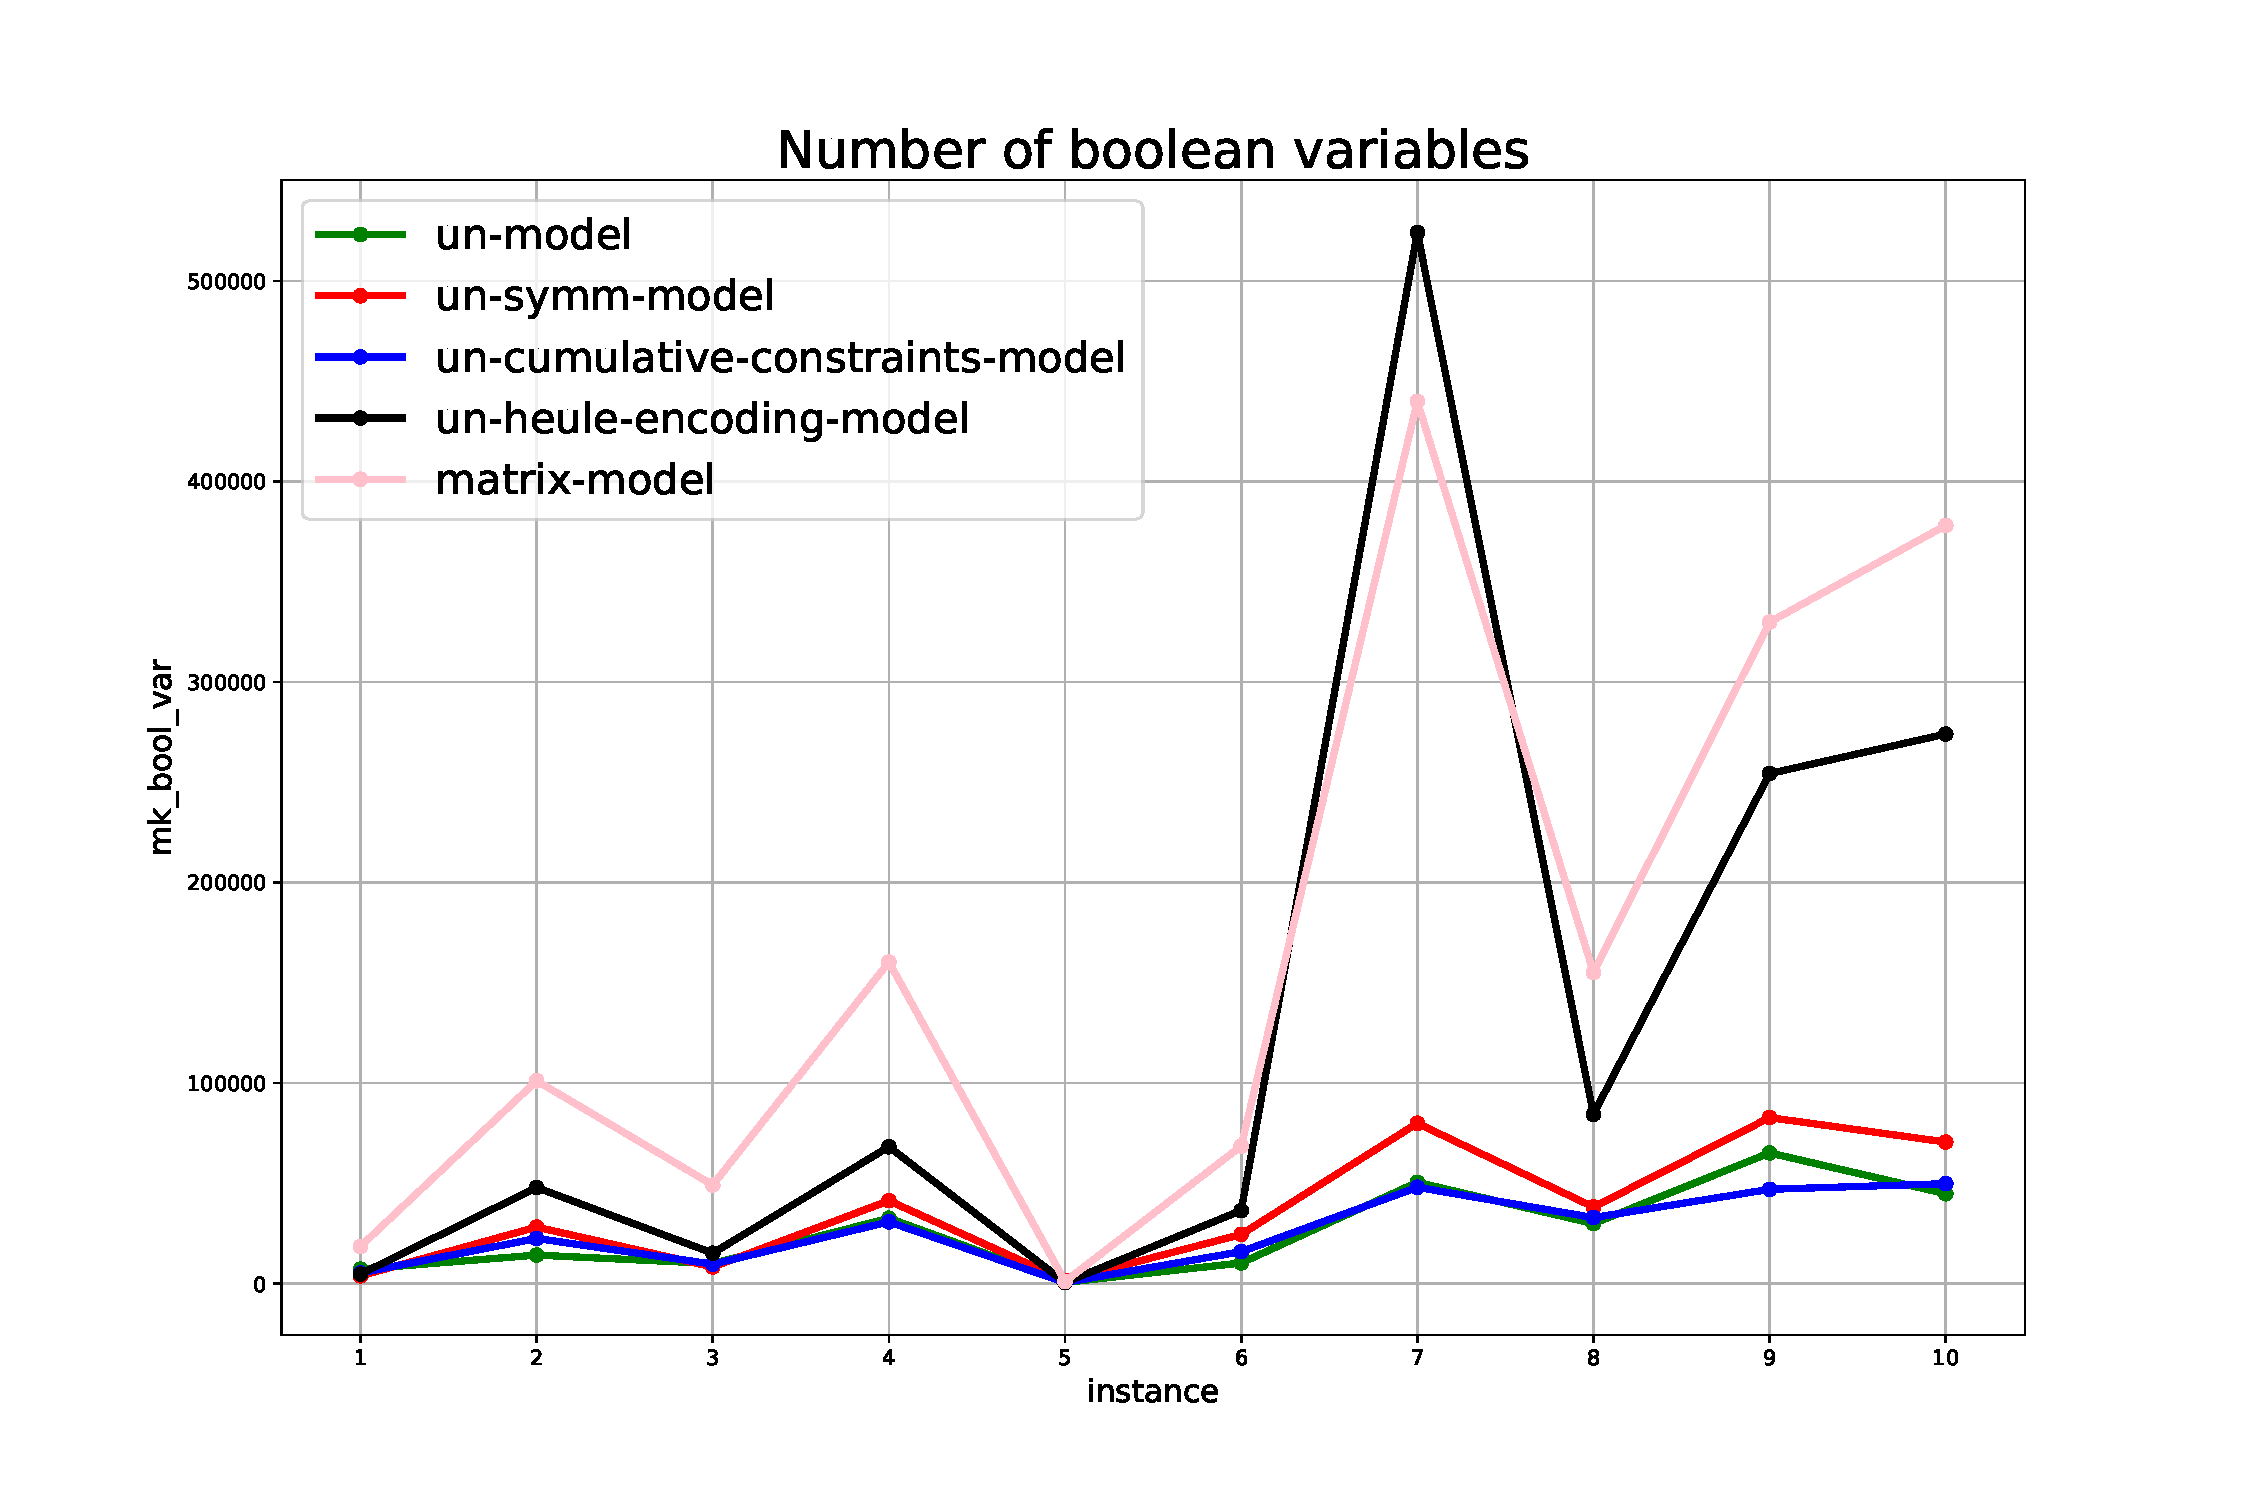
\includegraphics[width=\linewidth]{img/sat/mk_bool_var.pdf}
        % \caption{Number of boolean variables}
    % \end{subfigure}
    % \hfill
    % \centering
    % \hfill
    % \centering
    % \begin{subfigure}{0.49\linewidth}
    %     \centering
    %     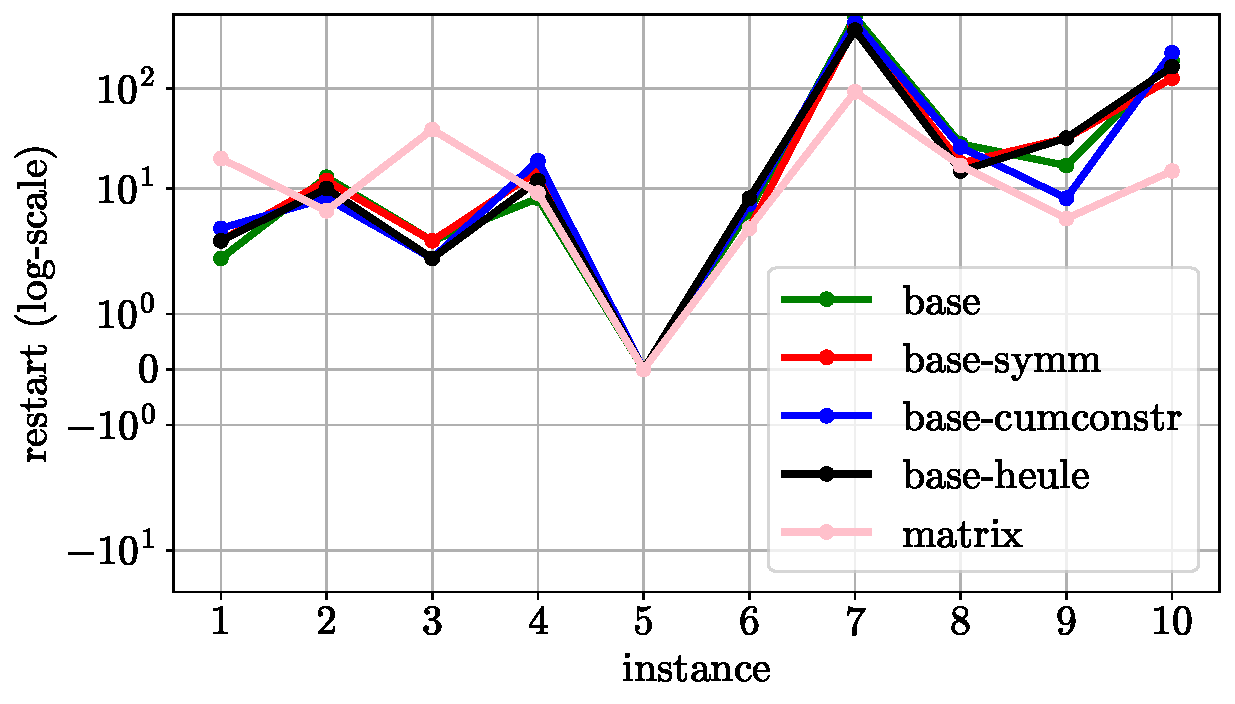
\includegraphics[width=\linewidth]{img/sat/restart.pdf}
    %     \caption{Number of restarts}
    % \end{subfigure}
    \caption{Statistics about the resolution of the problem for the first 10 instances}
    \label{fig:sat_plots}
\end{figure}

For all models, some statistics were extracted and are presented in \Cref{fig:sat_plots}:
\begin{enumerate*}[label=(\roman*)]
    \item \textit{time}: similar interval of time for all unified models variants, while the matrix model ensure in some instances a better performance;
    \item \textit{number of conflicts}: useful for estimating the size of the search space (the lower the better)\footnote{\url{https://stackoverflow.com/questions/17856574/how-to-interpret-statistics-z3}}. We can observe that the matrix model manage to have fewer conflicts, which is in line with its resolution time;
    \item \textit{max memory}: also in line with the previous observations, the matrix model tend to require less memory to solve the problem.
\end{enumerate*}
